

\tikzset{every picture/.style={line width=0.75pt}} %set default line width to 0.75pt        

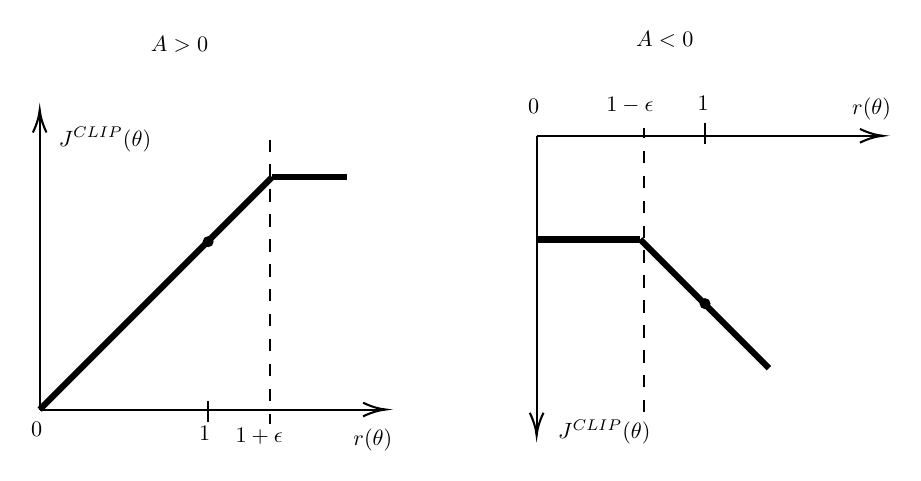
\begin{tikzpicture}[x=0.75pt,y=0.75pt,yscale=-1,xscale=1]
%uncomment if require: \path (0,283); %set diagram left start at 0, and has height of 283

%Straight Lines [id:da07428987415964317] 
\draw    (60.04,246.51) -- (60.04,104.1) ;
\draw [shift={(60.04,102.1)}, rotate = 450] [color={rgb, 255:red, 0; green, 0; blue, 0 }  ][line width=0.75]    (10.93,-3.29) .. controls (6.95,-1.4) and (3.31,-0.3) .. (0,0) .. controls (3.31,0.3) and (6.95,1.4) .. (10.93,3.29)   ;
%Straight Lines [id:da42162293191171707] 
\draw    (60.04,246.51) -- (224.76,246.51) ;
\draw [shift={(226.76,246.51)}, rotate = 180] [color={rgb, 255:red, 0; green, 0; blue, 0 }  ][line width=0.75]    (10.93,-3.29) .. controls (6.95,-1.4) and (3.31,-0.3) .. (0,0) .. controls (3.31,0.3) and (6.95,1.4) .. (10.93,3.29)   ;
%Straight Lines [id:da46857481861880057] 
\draw  [dash pattern={on 4.5pt off 4.5pt}]  (170.93,116.45) -- (170.93,253.43) ;
%Straight Lines [id:da5916594745882346] 
\draw [line width=2.25]    (60.04,246.51) -- (171.98,134.58) ;
%Straight Lines [id:da20769803027157696] 
\draw [line width=2.25]    (171.98,134.58) -- (208.01,134.58) ;
%Shape: Ellipse [id:dp9944817970164661] 
\draw  [fill={rgb, 255:red, 0; green, 0; blue, 0 }  ,fill opacity=1 ] (139.07,165.63) .. controls (139.07,164.46) and (140.02,163.51) .. (141.19,163.51) .. controls (142.36,163.51) and (143.31,164.46) .. (143.31,165.63) .. controls (143.31,166.8) and (142.36,167.75) .. (141.19,167.75) .. controls (140.02,167.75) and (139.07,166.8) .. (139.07,165.63) -- cycle ;
%Straight Lines [id:da631388526485618] 
\draw    (141.19,252.63) -- (141.19,242.51) ;
%Straight Lines [id:da5700736740675836] 
\draw    (299.45,114.62) -- (299.45,257.03) ;
\draw [shift={(299.45,259.03)}, rotate = 270] [color={rgb, 255:red, 0; green, 0; blue, 0 }  ][line width=0.75]    (10.93,-3.29) .. controls (6.95,-1.4) and (3.31,-0.3) .. (0,0) .. controls (3.31,0.3) and (6.95,1.4) .. (10.93,3.29)   ;
%Straight Lines [id:da4383859714024194] 
\draw    (299.45,114.62) -- (464.17,114.62) ;
\draw [shift={(466.17,114.62)}, rotate = 540] [color={rgb, 255:red, 0; green, 0; blue, 0 }  ][line width=0.75]    (10.93,-3.29) .. controls (6.95,-1.4) and (3.31,-0.3) .. (0,0) .. controls (3.31,0.3) and (6.95,1.4) .. (10.93,3.29)   ;
%Straight Lines [id:da15252831399229727] 
\draw [line width=2.25]    (349.38,164.55) -- (411.38,226.55) ;
%Straight Lines [id:da20676916509391385] 
\draw [line width=2.25]    (299.29,164.55) -- (349.38,164.55) ;
%Shape: Ellipse [id:dp5844715267834208] 
\draw  [fill={rgb, 255:red, 0; green, 0; blue, 0 }  ,fill opacity=1 ] (378.47,195.5) .. controls (378.47,196.67) and (379.42,197.62) .. (380.59,197.62) .. controls (381.77,197.62) and (382.72,196.67) .. (382.72,195.5) .. controls (382.72,194.33) and (381.77,193.38) .. (380.59,193.38) .. controls (379.42,193.38) and (378.47,194.33) .. (378.47,195.5) -- cycle ;
%Straight Lines [id:da16120535517562784] 
\draw    (380.59,108.5) -- (380.59,118.62) ;
%Straight Lines [id:da12247292832159551] 
\draw  [dash pattern={on 4.5pt off 4.5pt}]  (350.97,247.88) -- (350.97,110.91) ;

% Text Node
\draw (450.29,95.06) node [anchor=north west][inner sep=0.75pt]  [xscale=0.8,yscale=0.8]  {$r(\theta)$};
% Text Node
\draw (68.02,109.38) node [anchor=north west][inner sep=0.75pt]  [xscale=0.8,yscale=0.8]  {$J^{CLIP}( \theta )$};
% Text Node
\draw (135.61,253.59) node [anchor=north west][inner sep=0.75pt]  [xscale=0.8,yscale=0.8]  {$1$};
% Text Node
\draw (153.24,254.39) node [anchor=north west][inner sep=0.75pt]  [xscale=0.8,yscale=0.8]  {$1+\epsilon $};
\draw (210.0,254.87) node [anchor=north west][inner sep=0.75pt]  [xscale=0.8,yscale=0.8]  {$r(\theta)$};
% Text Node
\draw (112.41,65.43) node [anchor=north west][inner sep=0.75pt]  [xscale=0.8,yscale=0.8]  {$A >0$};
% Text Node
\draw (308.62,250.38) node [anchor=north west][inner sep=0.75pt]  [xscale=0.8,yscale=0.8]  {$J^{CLIP}( \theta )$};
% Text Node
\draw (375.82,94.26) node [anchor=north west][inner sep=0.75pt]  [xscale=0.8,yscale=0.8]  {$1$};
% Text Node
\draw (331.89,95.06) node [anchor=north west][inner sep=0.75pt]  [xscale=0.8,yscale=0.8]  {$1-\epsilon $};
% Text Node
\draw (294.15,95.86) node [anchor=north west][inner sep=0.75pt]  [xscale=0.8,yscale=0.8]  {$0$};
% Text Node
\draw (54.74,251.19) node [anchor=north west][inner sep=0.75pt]  [xscale=0.8,yscale=0.8]  {$0$};
% Text Node
\draw (346.2,63.03) node [anchor=north west][inner sep=0.75pt]  [xscale=0.8,yscale=0.8]  {$A< 0$};


\end{tikzpicture}